\documentclass[10pt,letterpaper]{article} 
\usepackage{cogsci} 
\usepackage{pslatex} 
\usepackage{apacite}
\usepackage{graphicx}
\usepackage{pdfsync}
\usepackage{natbib}


\title{Sources of developmental change in pragmatic inferences about scalar terms}

\author{{\large \bf Alexandra C. Horowitz} \\ \texttt{ahorowit@stanford.edu}\\ Department of Psychology \\ Stanford University \\ 
\And {\large \bf Michael C. Frank} \\ \texttt{mcfrank@stanford.edu} \\ Department of Psychology \\ Stanford University \\ }

\begin{document}

\maketitle

\begin{abstract} 

The ability to compute pragmatic implicatures---inferring that a weak statement (e.g. ``some of my siblings'') implies that a stronger statement (``all of my siblings'') could not be used---is a popular test case for children's pragmatic development. A growing body of work suggests that children can make implicatures under some conditions, but their performance varies widely across tasks, and few datasets allow direct comparisons between implicature types. To address this issue, we combine different types of implicatures and control trials into a single, simple paradigm. In Experiment 1, we included both ad-hoc (contextual) and scalar (quantifier) descriptions, and found that 4-year-olds were at ceiling in ad-hoc trials but had difficulty with scalar implicatures using quantifiers.  In Experiment 2, 4-year-olds' performance increased when we included only scalar trials, but was still low. Across both datasets, we found a positive correlation between performance on ``some'' and ``none'' trials. In addition to providing more precise developmental data on the emergence of different implicature computations, our work illustrates that preschoolers' recognition of implicatures relates both to their comprehension of particular descriptors used and also their recognition of relevant lexical alternatives. 



%replicated the finding that both ``some'' and ``none'' trials are difficult for yo ung children, and performance with these terms was bimodal and highly correlated. In a simple, supportive paradigm, our work illustrates that preschoolers' recognition of implicatures relates both to their comprehension of particular descriptors used, in addition their comparison with other possible lexical alternatives. 

{Keywords:} Pragmatics; implicature; language development. 
\end{abstract}

\section{Introduction}

Cooperative communicators tend to choose words that are informative about their intended meaning. For example, the use of a weak description (e.g. ``I did \textbf{some} of my homework'') implies that the stronger lexical alternative (that I did \emph{\textbf{all}} of my homework) is not true. Other generalized implicatures of this type include modals (\emph{possibly} versus \emph{definitely}), logical connectives (\emph{or} versus \emph{and}), and numerals (\emph{one} versus \emph{two}) \citep{horn1972}.  On the Gricean analysis \citep{grice1975}, the selection of a weaker scalar term (e.g. ``some'') implies that it would not have been truthful or accurate to use the stronger description (``all''), or else the speaker would have---hence, the listener is licensed in making an inference that the speaker did \emph{some but not all} of her homerwork. 

%These generalized implicatures are formed from the use of a weaker member of a lexical scale used in place of a stronger alternative, such as quantifiers (\emph{some} versus \emph{all}), modals (\emph{possibly} versus \emph{definitely}), logical connectives (\emph{or} versus \emph{and}), and numerals (\emph{one} versus \emph{two}) \citep{horn1984}.  On the Gricean analysis \citep{grice1975}, the selection of a weaker scalar term implies that a stronger one could not be used.  For example, stating that ``I completed \emph{some} of my homework'' conveys that it would not be truthful or accurate to use the stronger description that I completed \emph{all} of my homework.  If I had completed it all, I should have said so.  Because I used the weaker quantifier, \emph{some}, this implies that I completed some \emph{but not all} of the work.  

Children's processing of scalar implicatures has been a focal case study for pragmatic development. Although adults spontaneously compute scalar implicatures along lexical scales like $<$ {\sc some, all} $>$, children's performance is variable even fairly late in development \citep{noveck2001}.  Paradigms that require children to make truth judgments for complex propositions may underestimate their pragmatic abilities, however, and show a graded pattern of successes and failures across different tasks \citep{guasti2005,papafragou2003, papafragou2004}. For example, in one study, five-year-olds were able to evaluate the pragmatic felicity of quantifiers when they were given a ternary judgment task so that they could provide a medium size reward for true but pragmatically odd descriptions \citep{katsos2011}.  

Overall, research on children's abilities to compute scalar implicatures suggests that their fragile performance may have less to do with their general pragmatic knowledge per se, and more to do with their knowlege of the particular lexical scales being queried. The \emph{Alternatives Hypothesis}, proposed by Barner and colleagues \citep{barner2010, barner2011}, posits that children's ability to compute scalar implicatures relies on their recognition of the relevant scalar alternatives (e.g., that use of the weaker term ``some'' conveys a direct contrast with the stronger alternative ``all'', thus implying \emph{some \textbf{but not all}}).  In other words, children's pragmatic inferences rely on their ability to consider relevant possible alternative word choices that could have been used in place of the ones the speaker chose. So even in supportive paradigms, if children cannot bring to mind ``all'' when reasoning about ``some,'' they will fail to make an implicature.

Children's performance in implicature tasks increases when they have stronger access to lexical alternatives, supporting this hypothesis.  Evaluating performance in competitions where alternative outcomes are salient \citep{papafragou2003} and using contextually-accessible scales (e.g., ``the cat and the cow are sleeping'' rather than ``some animals are sleeping''; \cite{barner2011}) both help preschoolers make implicatures. 

The alternatives hypothesis also predicts interactions between with the type of task that is used and children's performance. For example, older three-year-olds show evidence of computing implicatures for particularized scales when the task is a forced choice between possible interpretations \citep{stiller2014}. And preschoolers also showed some preliminary evidence of making scalar implicatures with quantifiers in a similar forced-choice paradigm, albeit with prosodic support \citep{miller2005}. 

In sum, the Alternatives Hypothesis appears to provide a good account of soem of the pattern of preschoolers' successes and failures in pragmatic implicature teasks. Nevertheless, work to date has varied widely in the particular scales and tasks that were used, and the developmental samples are relatively small and often span several years. These concerns make it difficult to interpolate across findings and draw strong inferences about the contrasts between contextually-supported and scalar implicatures. Our current study aims to fill this gap. 

We designed a simple reference selection task in which children were asked to select with of three book covers they thought the experimenter was describing. Our design allowed us to a) fully counterbalance the instructions children heard across trials, including ad-hoc versus scalar descriptions as well as implicature versus unambiguous control targets, b) examine both within-subject patterns of responses as well as between-subject developmental patterns, and c) provide children with visual alternatives to help reduce the demands of the task.

In Experiment 1, we included both ad-hoc and scalar descriptions with implicature and control trials for each. Similarly to previous work \cite[e.g.,][]{stiller2014}, 4-year-olds performed well on ad-hoc trials; on scalar implicature trials, however, their performance was very low. In Experiment 2, we ran the same task but replaced the ad-hoc trials so that all of the descriptions included scalar quantifiers. We found developmental increases in performance from for each trial type, and higher performance on implicature trials for 4-year-olds in this scalar-only version of the task. In both experiments, there was a bimodal distribution of responses on scalar implicature trials and a strong predictive relationship between individuals' performance on ``some'' (scalar implicature) and ``none'' (scalar control) trials, suggesting that the ability to compute scalar implicatures may involve not only recognition of the stronger scalemate ``all,'' but rather both ends of the scale. Overall, our findings suggest that scalar implicatures are difficult for preschoolers even in supportive contexts, and stronger recognition of lexical alternatives boosts performance. 

%In our current work, we combine a range of implicatures within a single paradigm design to examine whether we find reliable within- and between-subjects developmental patterns predicted by the availability of lexical alternatives. 


%This is the first study is to use a single paradigm to test a battery of implicatures, allowing us to examine both within-subject differences in performance by implicature type, as well as compare between-subjects data to investigate whether similar developmental patterns emerge across different types of implicatures with age.  In Experiment 1, we show that 4-year-olds have no difficulty with 

\section{Experiment 1} 

\subsection{Methods}

\subsubsection{Participants}

A planned sample of 48 children was recruited from Bing Nursery School at Stanford University.  Participants were recruited from two age groups: 24 4.0- to 4.5-year-olds (M = 4;2) and 24 4.5- to 5.0-year-olds (M = 4;7). Two additional children were excluded for stopping the study early, and one was excluded due to experimenter error. 

\subsubsection{Stimuli}

Children were shown printed images of three book covers, each depicting four familiar items (see Figure \ref{fig:demo}). An initial training trial featured a single unique item on each cover. For each of the 18 test trials, one book contained four items of a kind (e.g. four dogs), one book contained a different set of four items (e.g. four cats), and one book contained two pictures of a previous set and two pictures of a different set (e.g. two cats and two birds). Each set of books featured a different set of familiar items. 


 \begin{table*} [t]
   \caption{Study designs for Experiments 1 and 2, using script examples for the trial set pictured in Figure \ref{fig:demo}.  \label{tab:scripts} } 
   \begin{center} 
     \begin{tabular}{lccccc} 
        %  & \multicolumn{4}{c}{} \\
                      \hline 
       \null   Condition  & Trial type & \# trials in Expt. 1 & \# trials in Expt. 2 & Statement: ``On the cover of my book, ...'' & Target   \\ 
       \hline  
            Scalar & implicature & 4 & 6 &  ``...some of the pictures are cats'' & B	 \\ 
          & all  & 2 &  6 & ``...all of the pictures are cats'' & C		                 \\
           & none  & 2 & 6 & ``...none of the pictures are cats'' & A			\\ 
               & unambiguous `some' 	&  2 &  & ``...some of the pictures are birds'' & B					        \\ 
	\hline
	    Adhoc       & implicature & 4 &  & ``...there are cats'' & C 		\\ 
	     & distractor & 2 &  & ``...there are dogs'' & A	     \\ 
          & comparison & 2 &  & ``...there are birds'' & B 	   \\
       \hline 
     \end{tabular} 
  \end{center}
 \end{table*}
 
\subsubsection{Procedures}

Participants were tested individually in a quiet room at their preschool.  The experimenter explained that they would be playing a game in which she would think about one of the three books on each page and give a clue about it. She emphasized that she would only give one clue for each page, so children were to make their best guess about which book she was describing based on that clue. A breakdown of the trial types and sample scripts is provided in Table \ref{tab:scripts}.

Children began the task with a training trial where each of the covers featured a single unique item (e.g. ``On the cover of my book, there's a TV'' and children chose between a book with a TV, a book with a sofa, and a book with a refrigerator).  Following this initial training, children saw 18 test trials with new sets of familiar items similar to the one depicted in Figure \ref{fig:demo}.  Children were instructed to point to the book they thought the experimenter was describing. If children pointed to more than one book or their response was unclear, they were reminded that the experimenter was talking about just one book, and asked to touch the one book they thought she meant.  

For ad-hoc trials, the experimenter described the book cover by naming the images pictured. Ad-hoc control trials (four total) referred to unambiguous targets (e.g. ``On the cover of my book, there are dogs/birds'', see Figure \ref{fig:demo}).  Ad-hoc implicature trials (four total) required an inference about the speaker's intended meaning: e.g. ``On the cover of my book, there are cats'' could potentially refer to either the book with only cats or the book with cats and birds, but the speaker's decision to describe only cats suggests that she is referring to the cover with all cats and no birds, or else she would have mentioned both types of animals. 

For scalar trials, the experimenter described the target using quantifiers. Scalar control trials (6 total) referred to unambiguous targets: two trials each using \emph{all} and \emph{none} (e.g.``On the cover of my book, all/none of the pictures are cats'') and two trials featuring an unambiguous referent of \emph{some} (e.g. ``On the cover of my book, some of the pictures are birds'').  On scalar implicature trials (four total), the experimenter used a weak quantifier in reference to the item pictured across two book covers (e.g. ``On the cover of my book, some of the pictures are cats''). Because the speaker used a weak quantifier, the implicature is that she must mean the cover with two cats and two birds, because if she had meant the cover with only cats, she would have use the stronger quantifier (\emph{all}) instead. 

Trials were presented in a fixed order, counterbalanced for target location and book triad positions.  The description condition (ad-hoc or scalar quantifier) and trial type (implicature or control) for each book set were randomized across participants. The conditions (ad-hoc or scalar) and trial types (implicature or control) were spaced as much as possible so that two trials of the same type never occurred twice in a row. Children enjoyed the task, responded quickly to the clues, and often made statements such as, ``I'm good at this!'' although they were not provided feedback about their selections. The test session took about ten minutes to complete.

\subsection{Results}

Children's performance on all trial types is shown in Figure \ref{fig:expt1} (responses were coded as correct on implicature trials if children chose the implicature-consistent target). Across all of the ad-hoc trial types, children were near ceiling in selecting the intended target. This finding replicates previous work indicating that preschoolers can compute ad-hoc implicatures \citep{stiller2014} in a new task, and suggests that children can make such inferences even in the presence of varied types of descriptions (control trials and scalar references). 

Children's performance on scalar trials was markedly different and much lower. We ran a logistic mixed effect model, predicting correct responses as the interaction of age, condition (ad-hoc or scalar) and trial type (implicature or control), with random effects of participant and trial type. Performance was marginally lower for scalar trials than ad-hoc trials ($\beta = -8.02$, $p =.09$), and there was a significant interaction between condition and trial type, such that performance was significantly worse on scalar implicature trials ($\beta = 16.45$, $p = .02$).  There was also a significant 3-way interaction between condition, trial type, and age, such that performance on scalar implicature trials decreased with age ($\beta = -4.16$, $p < .01$). There were no significant differences adding trial location (trials in the first half versus second half of the experiment), indicating that performance did not change throughout the course of the experiment.

Although children largely made correct choices on \emph{all} trials, their responses were more varied for \emph{some} and \emph{none} trials.  Examining their patterns of responses more closely, we ran Hartigan's dip test and found significant bimodal distributions for both \emph{some} ($D=.15$, $p<.0001$) and \emph{none} ($D=.20$, $p<.0001$) trials, indicating that individuals tended not to respond at chance, but either consistently correctly or incorrectly on these categories of trials. Additionally, children's success on \emph{some} and \emph{none} trials were highly correlated with each other ($r=-.47$, $p<.001$)\footnote{This correlation was also replicated in a pilot version of this task, n=22, $r=0.94$, $p<.0001$.} such that children who performed better on \emph{some} trials also tended to perform better on \emph{none} trials (see Figure \ref{fig:expt1scatterplot}). Performance on neither \emph{none} and \emph{all} trials ($r=.11$, $p=.45$) nor \emph{some} or \emph{all} trials ($r=.01$, $p=.95$) were correlated.

 \begin{figure}[h] 
  \begin{center} 
    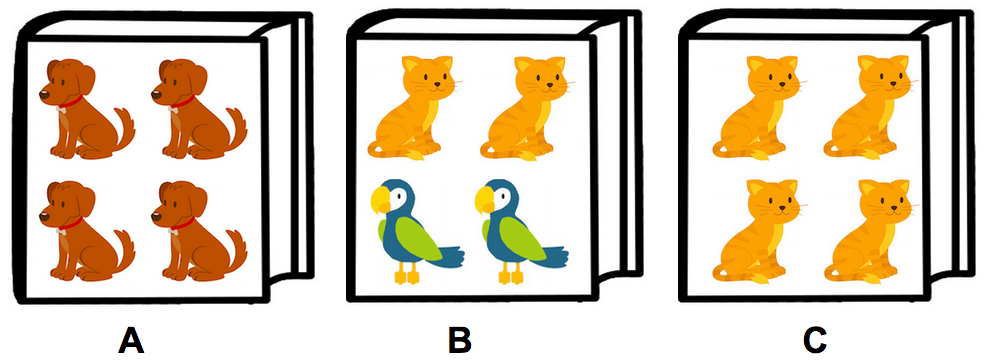
\includegraphics[width=3.5in]{figures/implicatures_demo_letters.png} 
    \caption{\label{fig:demo} Example trial image set. Children saw three book covers with familiar images. The experimenter provided a clue about which of the three covers she was thinking of, using either an ad-hoc or scalar description of either an unambiguous or implicature target (see scripts in Table \ref{tab:scripts}).}
    \end{center} 
%\vspace{-1ex} 
\end{figure}

\subsection{Discussion}

\begin{figure*}[t] 
  \begin{center} 
    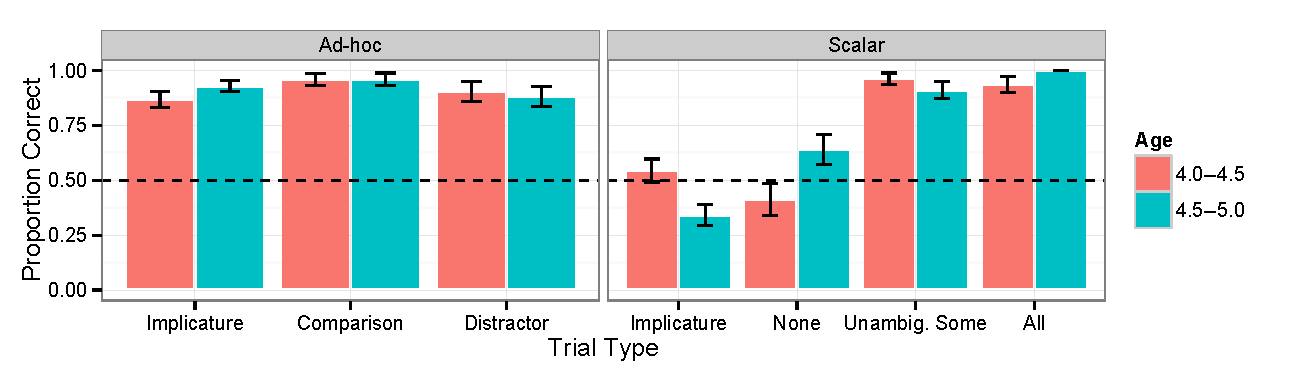
\includegraphics[width=7.5in]{figures/implicatures_adhocScalar_long.pdf} 
    \caption{\label{fig:expt1} Proportion of correct responses by age group for ad-hoc and scalar conditions in Experiment 1. Error bars show standard error of the mean.}
    \end{center} 
%\vspace{-1ex} 
\end{figure*}

\begin{figure}[h] 
  \begin{center} 
    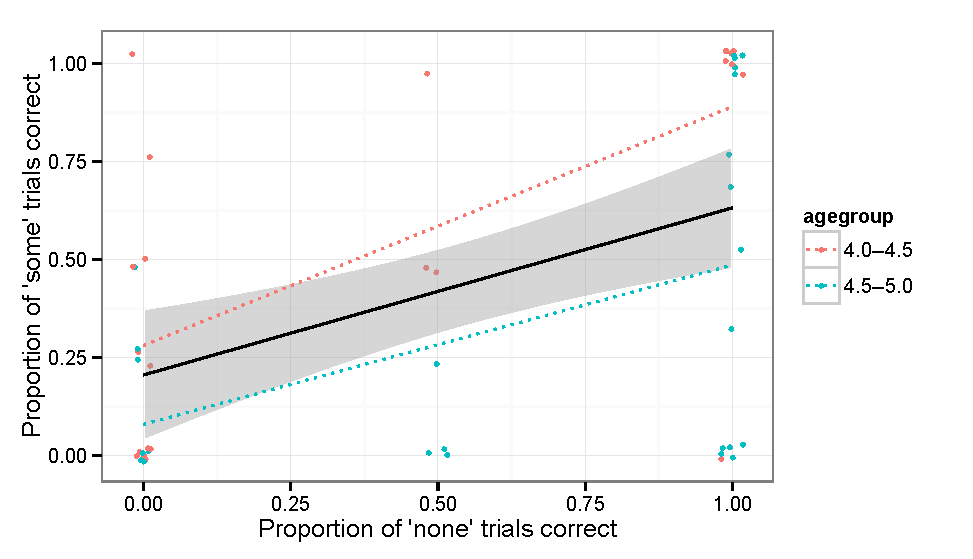
\includegraphics[width=3.3in]{figures/implicatures_adhocScalar_scatterplot.pdf} 
    \caption{\label{fig:expt1scatterplot} Scatterplot relating individuals' performance on \emph{some} trials and \emph{none} trials per age group in Experiment 1. The aggregate trend is plotted in black along with its 95\% confidence interval, and trends for each age group are shown by the dotted lines. Points are jittered slightly to avoid overplotting.}
    \end{center} 
%\vspace{-1ex} 
\end{figure}

%We were surprised by children's responses on scalar trials. 

Overall, we found that scalar implicatures were hard for children in our task. We wondered why this might be the case, given that we had tried to reduce as many task demands as possible in our task. Despite the presence of both visual alternatives (via the three selection choices) and lexical alternatives (conveyed across trials), children were at chance in their selections on scalar implicature trials. 

We also found an un-predicted developmental change in responses on \emph{none} trials, corroborating recent work by \cite{nordmeyer2014} indicating that even older preschoolers show difficulty in the comprehension of negation in arbitrary contexts. We had expected \emph{none} trials to serve as a simple unambiguous control, but found that this term was difficult for children (and that success was correlated with implicature performance). Perhaps children's implicature perfomance depends to some degree on familiarity with the both ends of the quantifier scale (\emph{none---some---all}). They may need to recognize both extremes of the scale before consistently identifying the meaning of the intermediate, \emph{some} term. Alternatively, another mediating factor (e.g., inhibitory control) might be responsible for the correlation we observed. We return to this issue in the General Discussion.

%Most previous work examines children's inferences about weak quantifiers (\emph{some}) compared with stronger alternatives (\emph{all}) without included the other end of the scale (\emph{none}).  

Finally, although a goal of our study was to examine pragmatic development by comparing children's performance across a variety of inference trials, we wondered if including \emph{both} ad-hoc and scalar quantifier descriptions led children to form expectations about the speaker that influenced their response. For instance, we were concerned whether their overwhelming success on ad-hoc implicature trials (e.g. ``On the cover of my book, there are cats'') might lead children to misinterpret the intention of ``some'' in scalar implicature trials from ``On the cover of my book, some of the pictures are cats'' to ``On the cover of my book, there are some cats.'' If children are forming expectations about the speaker that override their sensitivity to the particular word choices in the referential expression, then their performance may be biased by the presence of the ad-hoc trials.  To investigate this idea, we removed ad-hoc trials and ran a scalar-only version of the study in Experiment 2.

\section{Experiment 2} 

%In Experiment 1, we examined preschooler's sensitivity to speakers' descriptive choices by combining ad-hoc and scalar quantifier descriptions into a single, supportive task. We found that children had no trouble with ad-hoc control or implicature trials, but they did have difficulty with scalar implicature trials and descriptions involving \emph{none}. Although we tried to reduce as many task demands as possible by having children select the speaker's referent from visual alternatives, these simplified paradigm was still a challenge for children's ability to compute scalar implicatures. 

To investigate whether preschoolers would show increased sensitivity to individual quantifier use in the absence of competing ad-hoc descriptions, we ran a version of the task in which all 18 trials featured scalar quantifiers in Experiment 2. Additionally, in order to explore the developmental course of scalar implicature comprehension, we extended our sample to span the age range from 3--5 years, broken into half-year age groups.

\subsection{Methods}

\subsubsection{Participants}

We recruited a new sample of participants from Bing Nursery School, broken into half-year age groups: 12 3.0--3.5 year-olds (M=3;4), 12 3.5--4.0 year-olds (M=3;8), 14 4.0--4.5 year-olds (M=4;3), and 12 4.5--5.0 year-olds (M=4;8).  One additional child was excluded for stopping the task early. 

\subsubsection{Stimuli}

The same materials were used as in Experiment 1. The only changes made were to the scripts, such that ad-hoc trials were removed and all trials were converted into scalar quantifier references (Table \ref{tab:scripts}).  The 18 test trials contained six control \emph{all} trials (e.g. ``On the cover of my book, all of the pictures are cats''), six control \emph{none} trials (``On the cover of my book, none of the pictures are cats''), and six scalar implicature \emph{some} trials (``On the cover of my book, some of the pictures are cats'').  Trials were presented in a fixed order, counterbalanced for target location and triad order.  There were three scripts to which participants were randomly assigned, with each trial type (\emph{all, none} or \emph{some}) occurring once for each book set across the lists, and with a pseudo-randomized trial order such that participants never heard the same trial type twice in a row. 

\subsubsection{Procedures}

The procedure was identical to Experiment 1. 

\subsection{Results}

The proportion of correct trials by age group and trial type is shown in Figure \ref{fig:expt2}.  Children's performance increased with age for all trial types. All age groups were strongest on the \emph{all} trials, and the oldest children (4.5--5.0 year-olds) were the only age group above chance for all trial types.  T-TESTS

We ran a logistic mixed effect model, predicting correct responses as the interaction of age and trial type (\emph{none, some} or \emph{all}), with random effects of participant and trial type. The only significant effect that emerged was age, such that performance increased across trials as children got older ($\beta = 3.80$, $p < 0.001$). We added trial order (first or second half of the experiment) to this model but it did not interact with any variables, indicating that performance did not change over the course of the experiment.

Although 4-year-olds' performance increased on \emph{some} and \emph{none} trials with the scalar-only descriptions of Experiment 2, children overall had more difficulty with these trials than \emph{all} trials. There was a positive correlation between performance on \emph{all} and \emph{none} trials ($r=.47$, $p<.001$), indicating that children were  improving across both trial types with age.  There was no relationship between success on \emph{all} and \emph{some} trials ($r=-.03,$, $p=.83$), suggesting that comprehension of ``some'' was less systematic with age. We also still found significant bimodal patterns of responses for both \emph{some} ($D=.12$, $p<.0001$) and \emph{none} ($D=.15$, $p<.0001$) trials, and individuals' performance on \emph{none} and \emph{some} trials were highly correlated ($r=.52$, $p<.001$) (see Figure\ref{fig:expt2scatterplot}). 

\subsection{Discussion}

Our results suggest that children's ability to interpret scalar quantifiers is largely driven by their familiarity with these terms, which is highly related to age. Overall, children's success in selecting the speaker's intended target increased as children got older, perhaps driven by their knowledge of quantifier terms, or due to their sensitivity to pragmatic implications of word choice more generally. The bimodal and predictive pattern of responses for both \emph{none} and \emph{some} terms, and simultaneous near ceiling performance on \emph{all} trials, suggests that children may be developing a specific understanding of quantifier use in their preschool years. They may be learning that both \emph{none} and \emph{some} contrast with \emph{all} in parallel, as evidenced by their systematic responses to these trials. Finally, there was a notable contrast between performance on \emph{some} trials in Experiment 1 and Experiment 2, indicating that the presence of other trial types likely decreased children's implicature computation. 

% Each of the three quantifier types (\emph{all, some}, and \emph{none}) occurred in six trials spaced throughout Experiment 2, so a highly correlated, bimodal pattern of responses between \emph{none} and \emph{some} trials indicates reliable success or failure in processing the precise meanings of these terms in contrast to \emph{all}.


\begin{figure}[t] 
  \begin{center} 
    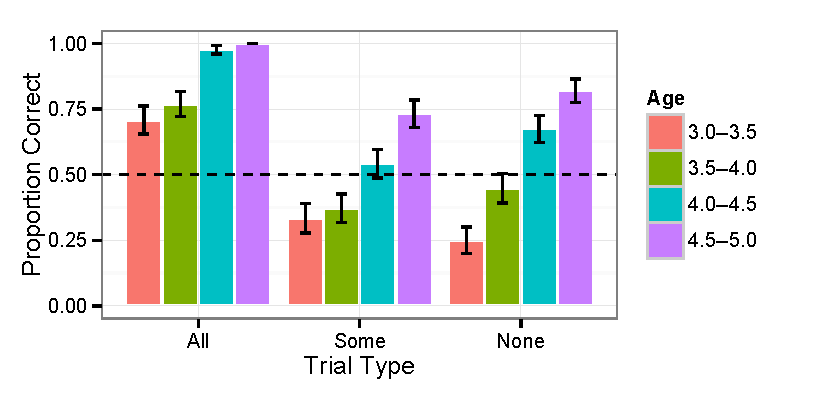
\includegraphics[width=3.5in]{figures/implicatures_scalarOnly_clean.pdf} 
    \caption{\label{fig:expt2} Proportion correct responses per age group for each of the scalar trial types (\emph{all, some} and \emph{none}) in Experiment 2. Error bars show standard error of the mean. }
    \end{center} 
\vspace{-1ex} 
\end{figure}

\begin{figure}[h] 
  \begin{center} 
    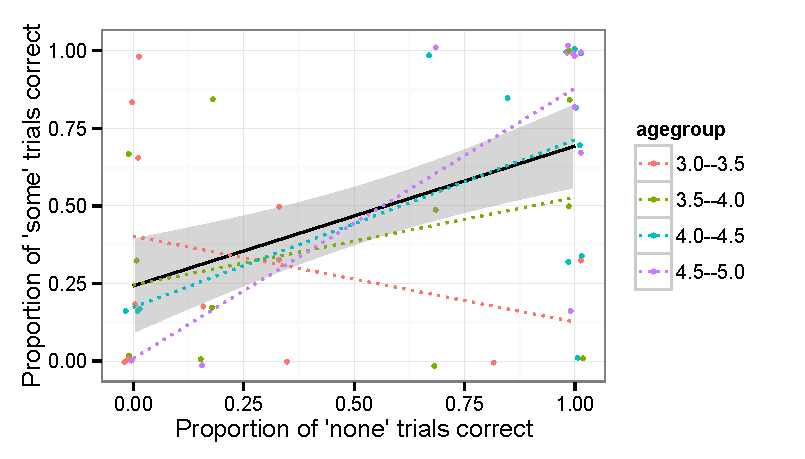
\includegraphics[width=3.3in]{figures/implicatures_scalarOnly_scatterplot.pdf} 
    \caption{\label{fig:expt2scatterplot} Scatterplot of individuals' performance on \emph{some} trials and \emph{none} trials in Experiment 2 (main effect in black, correlations per age groups illustrated by the dotted lines). Points are jittered slightly to avoid overplotting. }
    \end{center} 
\vspace{-1ex} 
\end{figure}


 \section{General Discussion} 
 
We designed a simple task to test children's sensitivity to a variety of word choice cues in a single paradigm, allowing us to investigate patterns of development both within- and between-subjects. We minimized task demands by using a reference selection context among three visual alternatives. In Experiment 1, we replicated the finding that preschoolers are strong at computing ad-hoc implicatures, and they were also at ceiling on unambiguous ad-hoc control trials. In Experiment 2, preschoolers' comprehension of all scalar terms in the task increased with age, and removing the ad-hoc trials increased older children's performance on \emph{some} and \emph{none} trials. Our findings suggest that 4-year-olds are able to compute scalar implicatures, but their performance is fragile and relies on strong contextual cues. 

Our work contributes to the existing literature in a number of ways. First, it offers a novel paradigm that is less complicated than many other implicature tasks, leading us to feel more confident that our results reflect children's true sensitivity rather than inadvertent difficulties of challenging task demands. Each test set remained visible to children, and they were merely asked to select which picture they thought was the referent of the speakers' description, which was randomized across trials. Second, the relatively high number of trials both helped strengthen our analytical power, and also offered the possibility for children to identify lexical alternatives as the study progressed (although we did not find that their performance significantly changed over the course of either experiment, cf. \cite{skordos2014}). Third, we were able to not only compare performance across age groups, but also examine individual patterns of responses across the different trial types. This design helped us determine that preschoolers' performance on scalar implicature trials was bimodal, and highly related to their performance on \emph{none} trials, which we would have been unlikely to uncover in a purely between-subjects implicature design without controls. 

Our findings are supportive of the Alternatives Hypothesis \cite{barner2010,barner2011}. First, our ad-hoc trials in Experiment 1 show that preschoolers had no difficulty making inferences about contextual descriptions generally when they are obvious from the context. Performance on scalar trials also appeared to be related to the recognition of alternatives, due to both preschoolers' increasing ability to compute scalar implicatures with age (presumably a proxy for familiarity with scalemates) and due to the difference in performance across Experiments 1 and 2. 

The correlated responses for \emph{some} and \emph{none} trials in both Experiments 1 and 2 indicates that children's inferences are also related to their comprehension of related lexical alternatives. \emph{None} is not typically considered part of the same Horn scale as \emph{some} and \emph{all} (because ``all'' entails \emph{some}, but ``some'' does not entail \emph{none}---and in fact entails the opposite), but it is nonetheless a lexical contrast along the same quantifier scale. INHIBITORY CONTROL? Overall, these patterns of results support the idea that children's ability to compute implicatures relates to their ability to consider what other possible utterance choices a speaker could have used instead.  







%though suggests that there may be more to the picture of children's ability to compute scalar implicatures. Our ad-hoc trials in Experiment 1 indicate that preschoolers had no difficulty making inferences about contextual descriptions, giving support that they evaluated the speaker's intended meaning when able to consider the possible descriptive choices for the visual alternatives; children tailored their selections to the speaker's most likely referent based on her choices of words given the potential items to be named in the scene. 

%For the scalar trials, we also see evidence that performance was based on recognition of lexical alternatives: preschoolers' ability to compute scalar implicatures increases with age (presumably a proxy for familiarity with these scalemates). Additionally, the correlated bimodal pattern of responses for \emph{some} and \emph{none} trials in both Experiments 1 and 2 indicates that children's inferences are related to their comprehension of related lexical alternatives. \emph{None} is not typically considered part of the same Horn scale as \emph{some} and \emph{all} (because ``all'' entails \emph{some}, but ``some'' does not entail \emph{none}---and in fact entails the opposite), but it is nonetheless a lexical contrast along the same quantifier scale. Overall, these patterns of results support the idea that children's ability to compute implicatures relates to their ability to consider what other possible utterance choices a speaker could have used instead.  As children gain more experience with language and members of the same quantifier scale, they are more likely to succeed in making inferences about the implications of these particular word choices. 


A pattern more difficult to reconcile with the Alternatives Hypothesis is the finding that children's performance did not change over the course of the experiments. We had expected that, if children were sensitive to opportunities for inferences based on contrasts in lexical choices, that their level of implicature performance should improve over the course of the experiment. In other words, because children comprehend ``all,'' they should infer that the speaker's choice to use ``all'' in some trials but ``some'' and ``none'' in others implies that she intends a reference other than \emph{all} by these alternative descriptions. This logic could be a purely a lexical inference (that ``all'' and ``some'' or ``none'' should not overlap in meaning), or a pragmatic inference (that if the speaker has selectively used ``all'' on certain trials and uses ``some'' or ``none'' on other trials, she probably intended a different meaning by using these different terms). Either route to inference should make children more likely to select the picture that is \emph{not} ``all'' on ``some'' and ``none'' trials, leading to an increase in correct target selections for ``some.'' The lack of trial order effects we observed may indicate that children do not yet have strong enough comprehension of these terms, do not recognize them as lexical alternatives, or do to perceive descriptive changes as indicators of contrast relevant to the context \citep{skordos2014}. The simple pictures in our task may have also influenced children's ability to interpret the speaker's descriptions, as adults rate quantifier use for small numbers as less natural than for larger numbers \citep{degen2014b}. 


%Because we don't see a change in performance across trials, it may be the case that children need stronger lexical knowledge of particular terms before making inferences purely on contrastive word choice. It may not be enough just to hear that a speaker is using different words, and may be the case that children need more evidence about the particular meanings of these terms before they can demonstrate inferences about changes in their implied meaning. 


%In other words, even if children were not complete comprehenders of ``some'' and ``none'', they should realize that, across the first few trials, that if they know the meaning of \emph{all} (at which they perform near ceiling), then they should be able to make the inference that a change in quantifier (``some'' or ``none'' in place of ``all'') should indicate a change in meaning (that another quantifier should not \emph{also} refer to the picture of \emph{all}).  

% In sum, sensitivity to speaker's word choices can facilitate the information exchange between conversational patterers. 
% Implicatures are particularly useful instances of pragmatic inferences because they involve \emph{implied} meaning, offering opportunities for a inference with high likelihoods of success when recognized compared with more subtle uses of language. 
Our work suggests that children can draw implicatures based on some lexical choices---such as in the case of ad-hoc implicatures---but they still struggle with quantifier-based scalar implicatures until relatively late. Their computation of scalar implicatures increases in supportive contexts, but their inferences are fragile and depend on their knowledge of lexical items.
% than the pragmatic cues of varying descriptive choices. Children may need to have a stronger comprehension of a lexical category before making inferences about possible within-category distinctions word choices convey.  Once they can recognize the relevant category contrasts intended, they can compute implicatures from these word choices. 

\section{Acknowledgments}

Special thanks to the Bing Nursery School, and Sara Altman and Carson Kautz for their help with data collection. 

\bibliographystyle{apacite}

\setlength{\bibleftmargin}{.125in} \setlength{\bibindent}{-\bibleftmargin}

\bibliography{implicatures}

\end{document}

